\section{Results}
\label{sec:results}

\TODO{Introduce}


\subsection{Repo-level analysis}
\label{sec:results1}

\TODO{Graphics placement}

This subsection focuses solely on repository-level analysis of our metrics, since comparison between individual commits and or individual authors would be tedious. Also, author-level analysis is open to everyone through the web interface.

\begin{figure}[p]
    \centering
    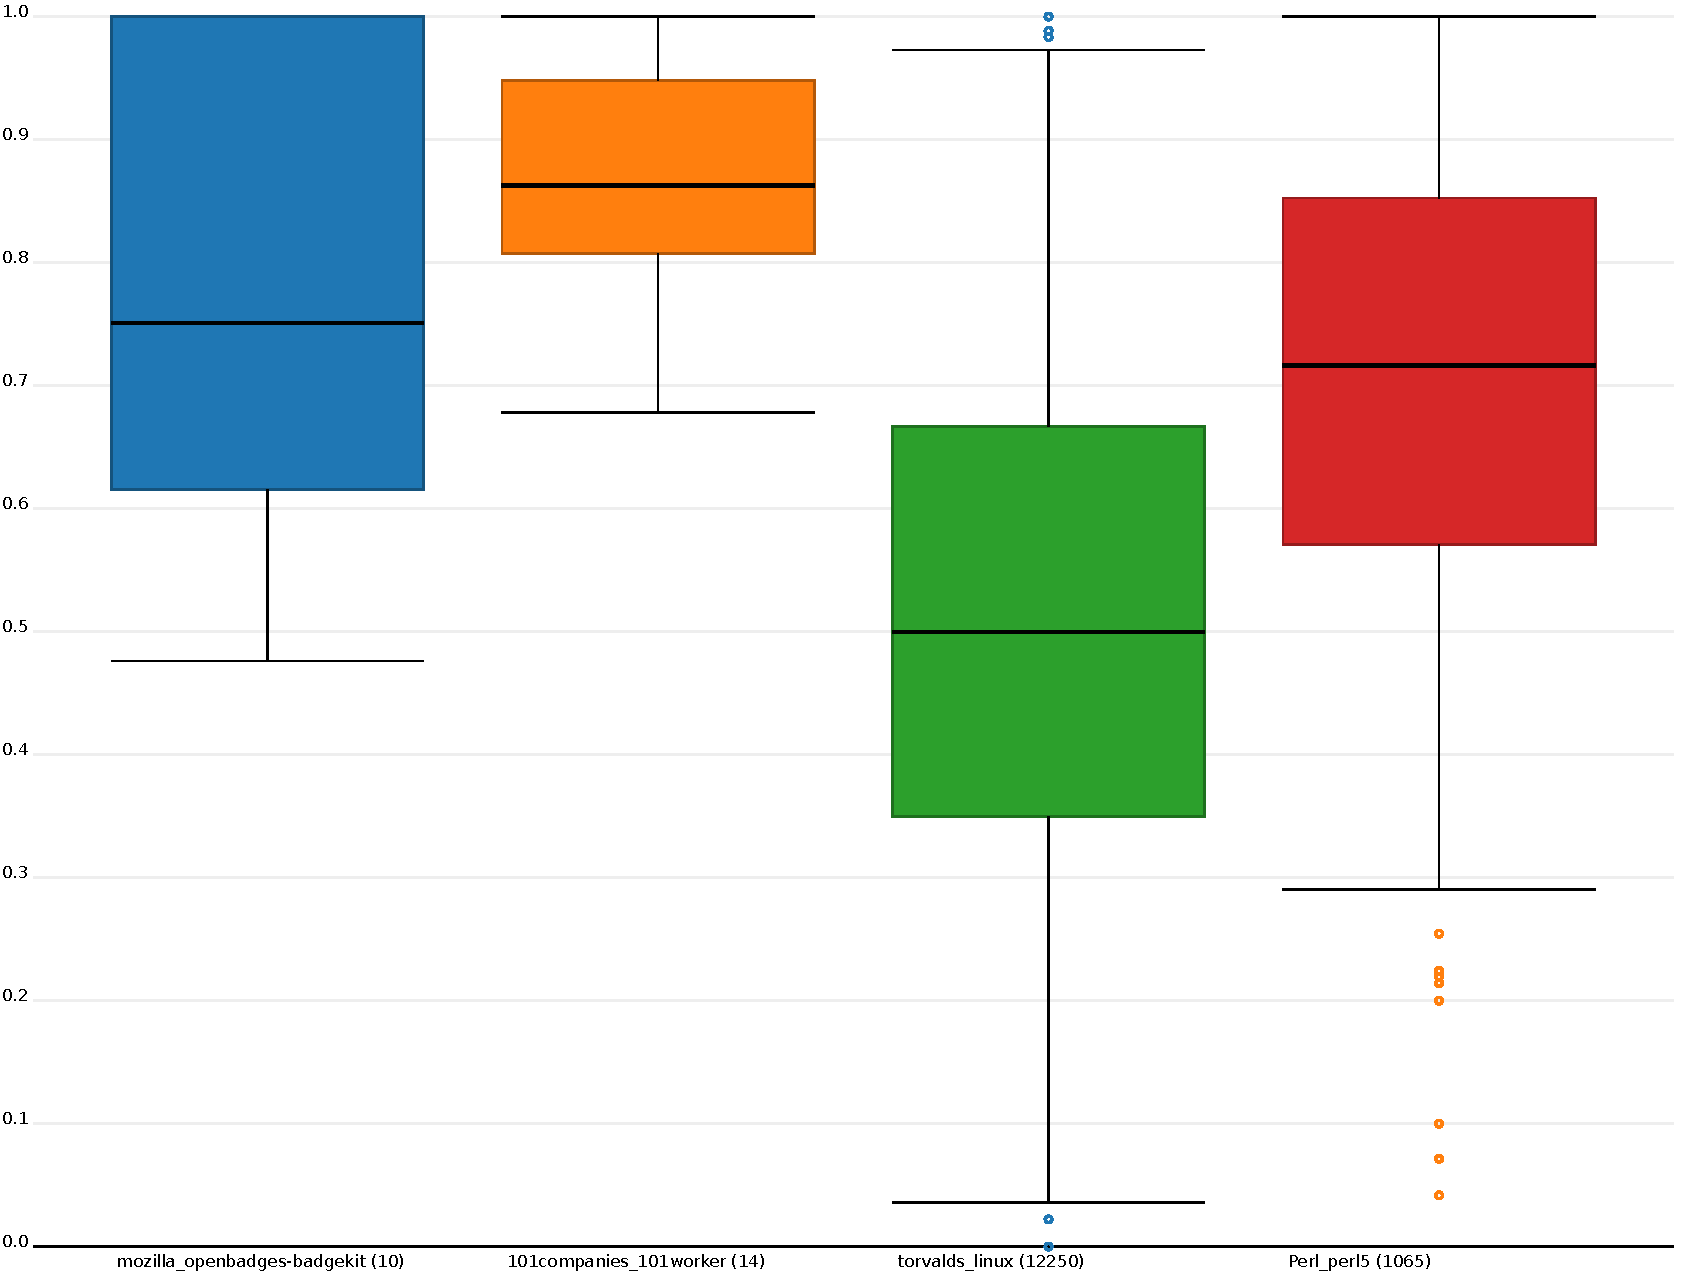
\includegraphics[width=0.8\textwidth]{img/subject_limit.pdf}
    \caption{Subject Limit Boxplot}
    \label{fig:bp_subject_limit}
\end{figure}

Figure \ref{fig:bp_subject_limit} shows the repository-level boxplots for the subject limit criterion for all 4 repositories. The number behind the labels denotes the number of authors that were evaluated in the graph. Surprisingly, the linux kernel has the worst results, followed by the badgekit and the perl5 and then the 101worker with the best results.

\begin{figure}[p]
    \centering
    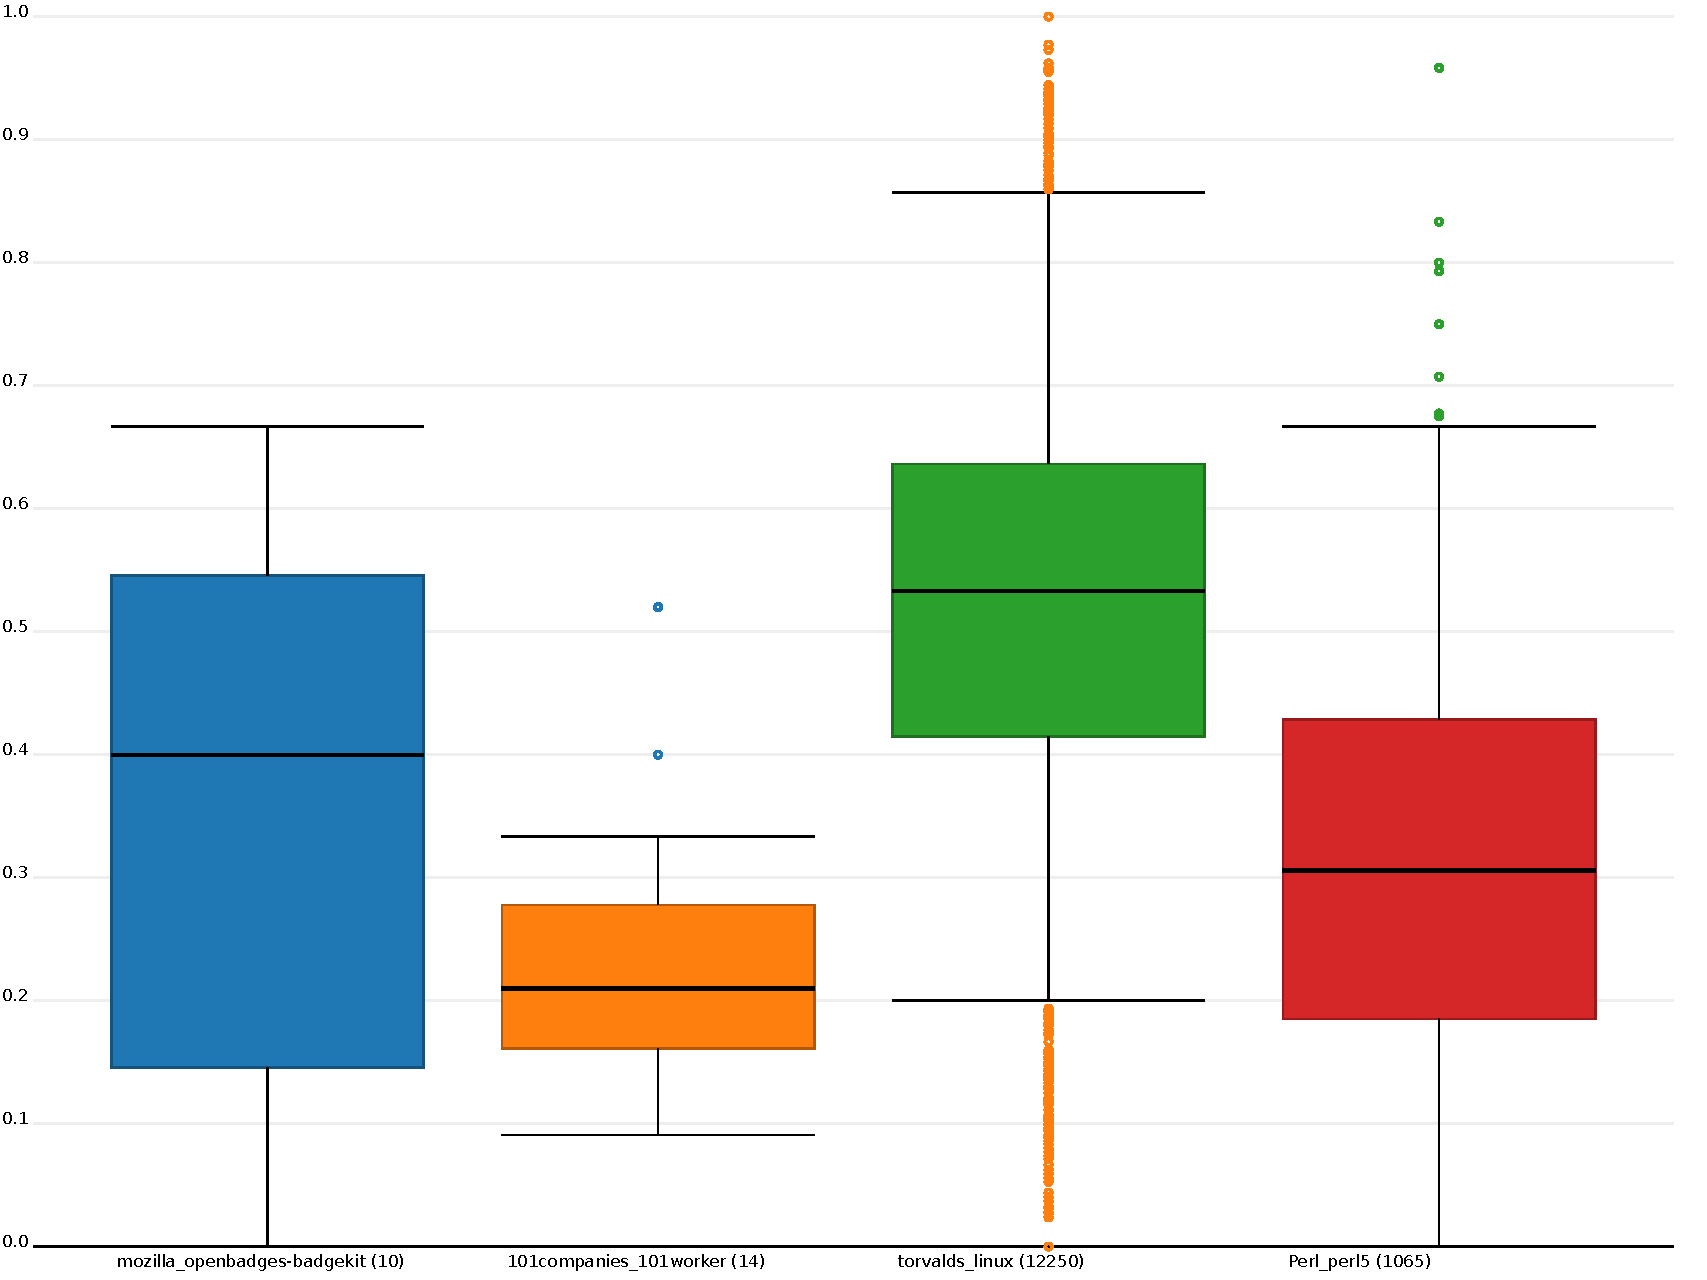
\includegraphics[width=0.8\textwidth]{img/imperative_subject.pdf}
    \caption{Imperative Subject Boxplot}
    \label{fig:bp_imperative_subject}
\end{figure}

\begin{figure}[p]
    \centering
    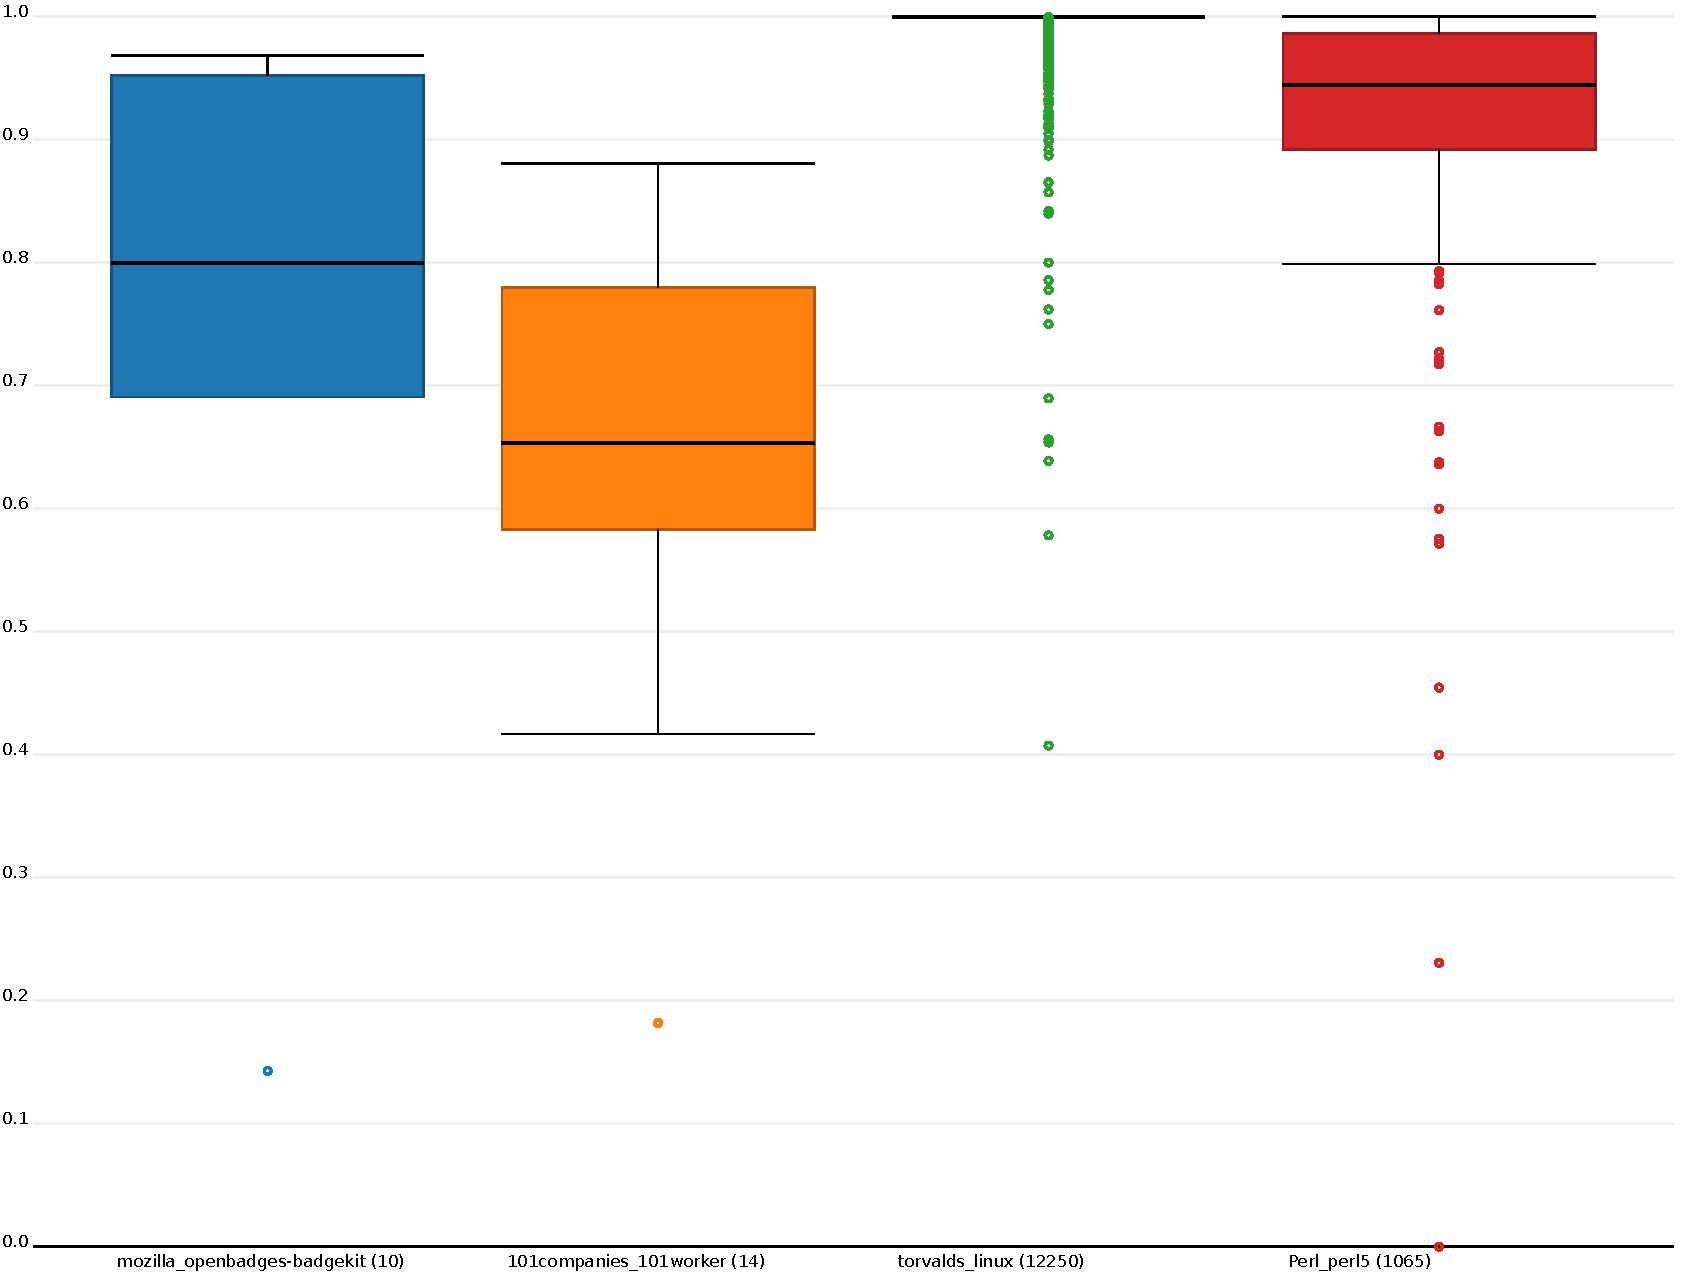
\includegraphics[width=0.8\textwidth]{img/no_short_message.pdf}
    \caption{No Short Message Boxplot}
    \label{fig:bp_no_short_message}
\end{figure}

On the other hand, figure \ref{fig:bp_imperative_subject} shows that authors of the linux kernel use the imperative mood for the subject the most, while the authors of the 101worker rarely do. Additionally, figure \ref{fig:bp_no_short_message} shows that linux kernel authors do not write short commit messages, while the authors of the 101worker do. This observation coincides with our estimations for the worker, since that criterion was inspired by a prevalence for 1-word commits in that repo.

\begin{figure}[p]
    \centering
    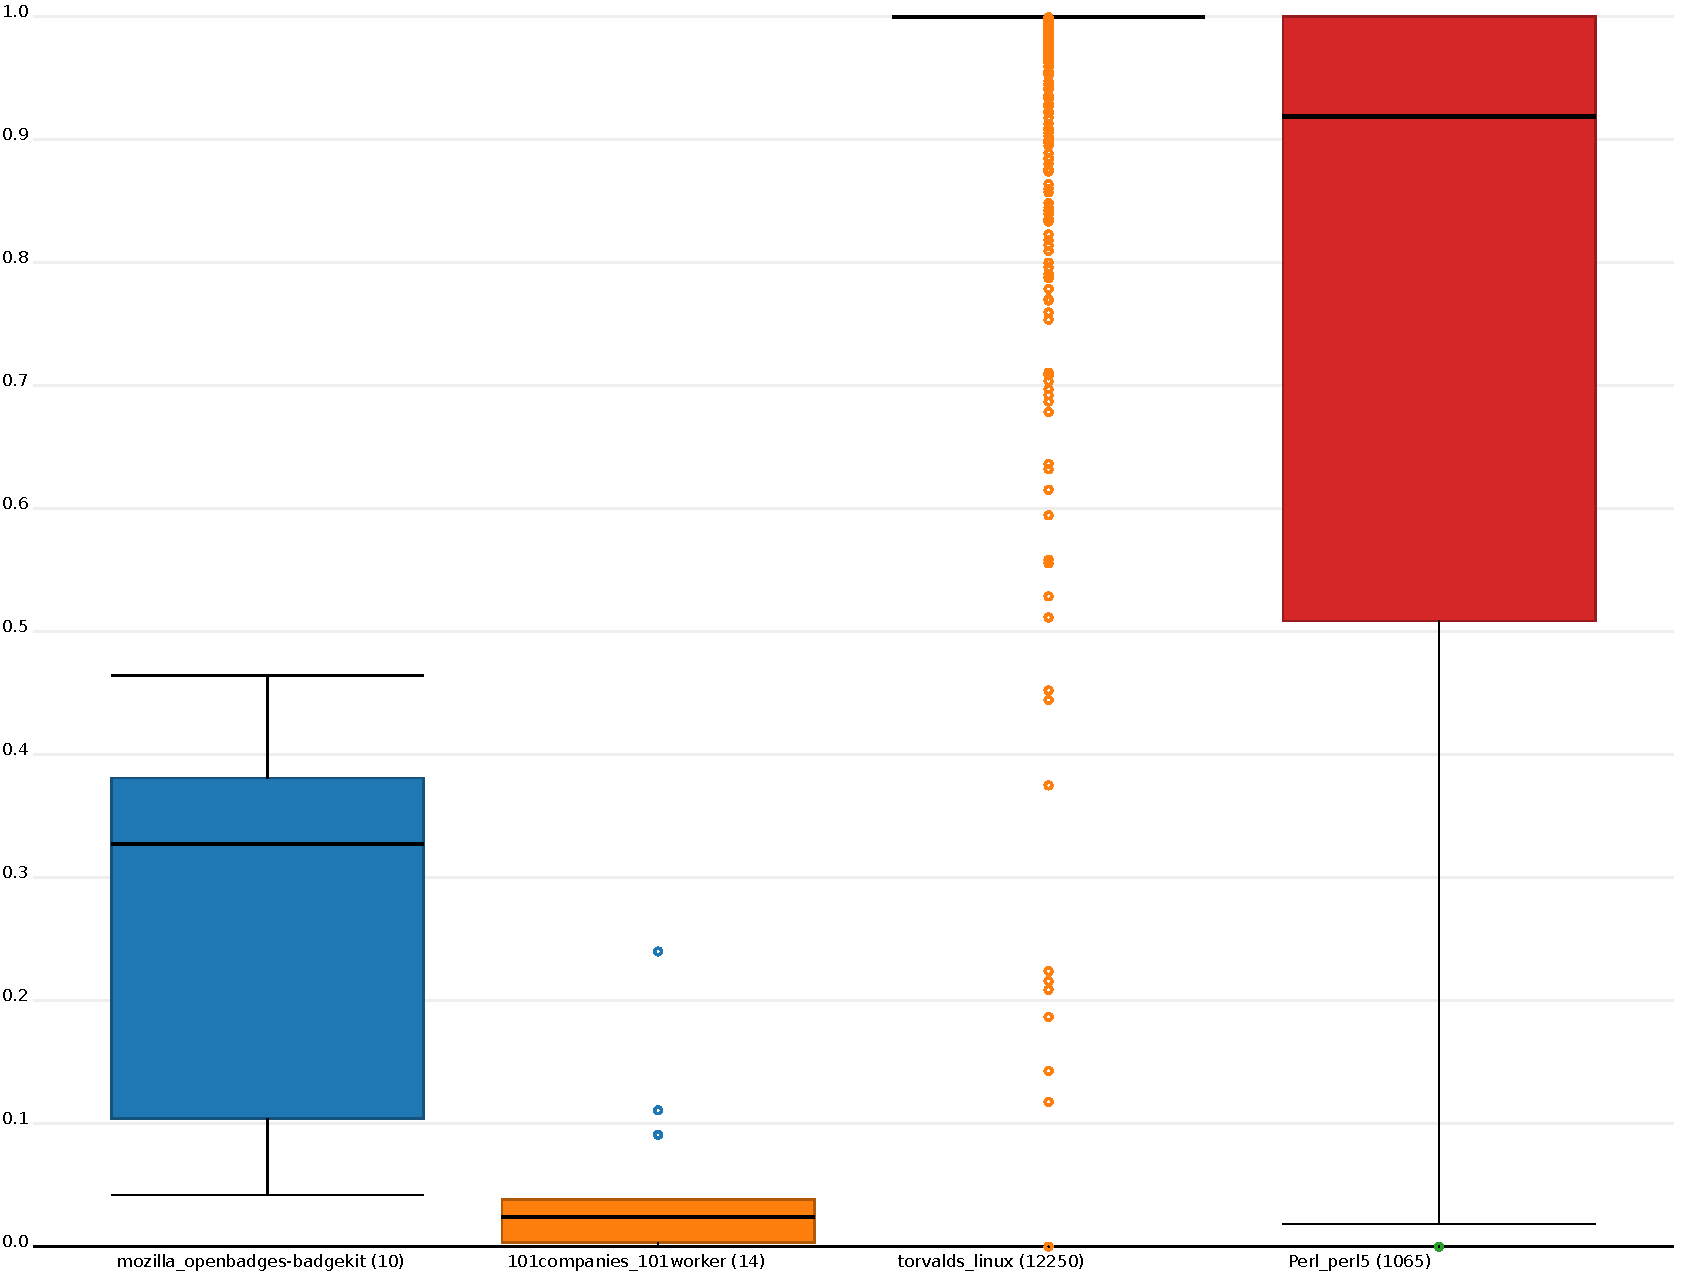
\includegraphics[width=0.8\textwidth]{img/body_used.pdf}
    \caption{Body Used Boxplot}
    \label{fig:bp_body_used}
\end{figure}

One significant difference between the two small repos (badgekit and 101worker) and the big repos (perl and linux kernel) stands out in figure \ref{fig:bp_body_used}. The big repos both make heavy use of the body, while it is almost never used by the worker and only sometimes by the badgekit.

\begin{figure}[p]
    \centering
    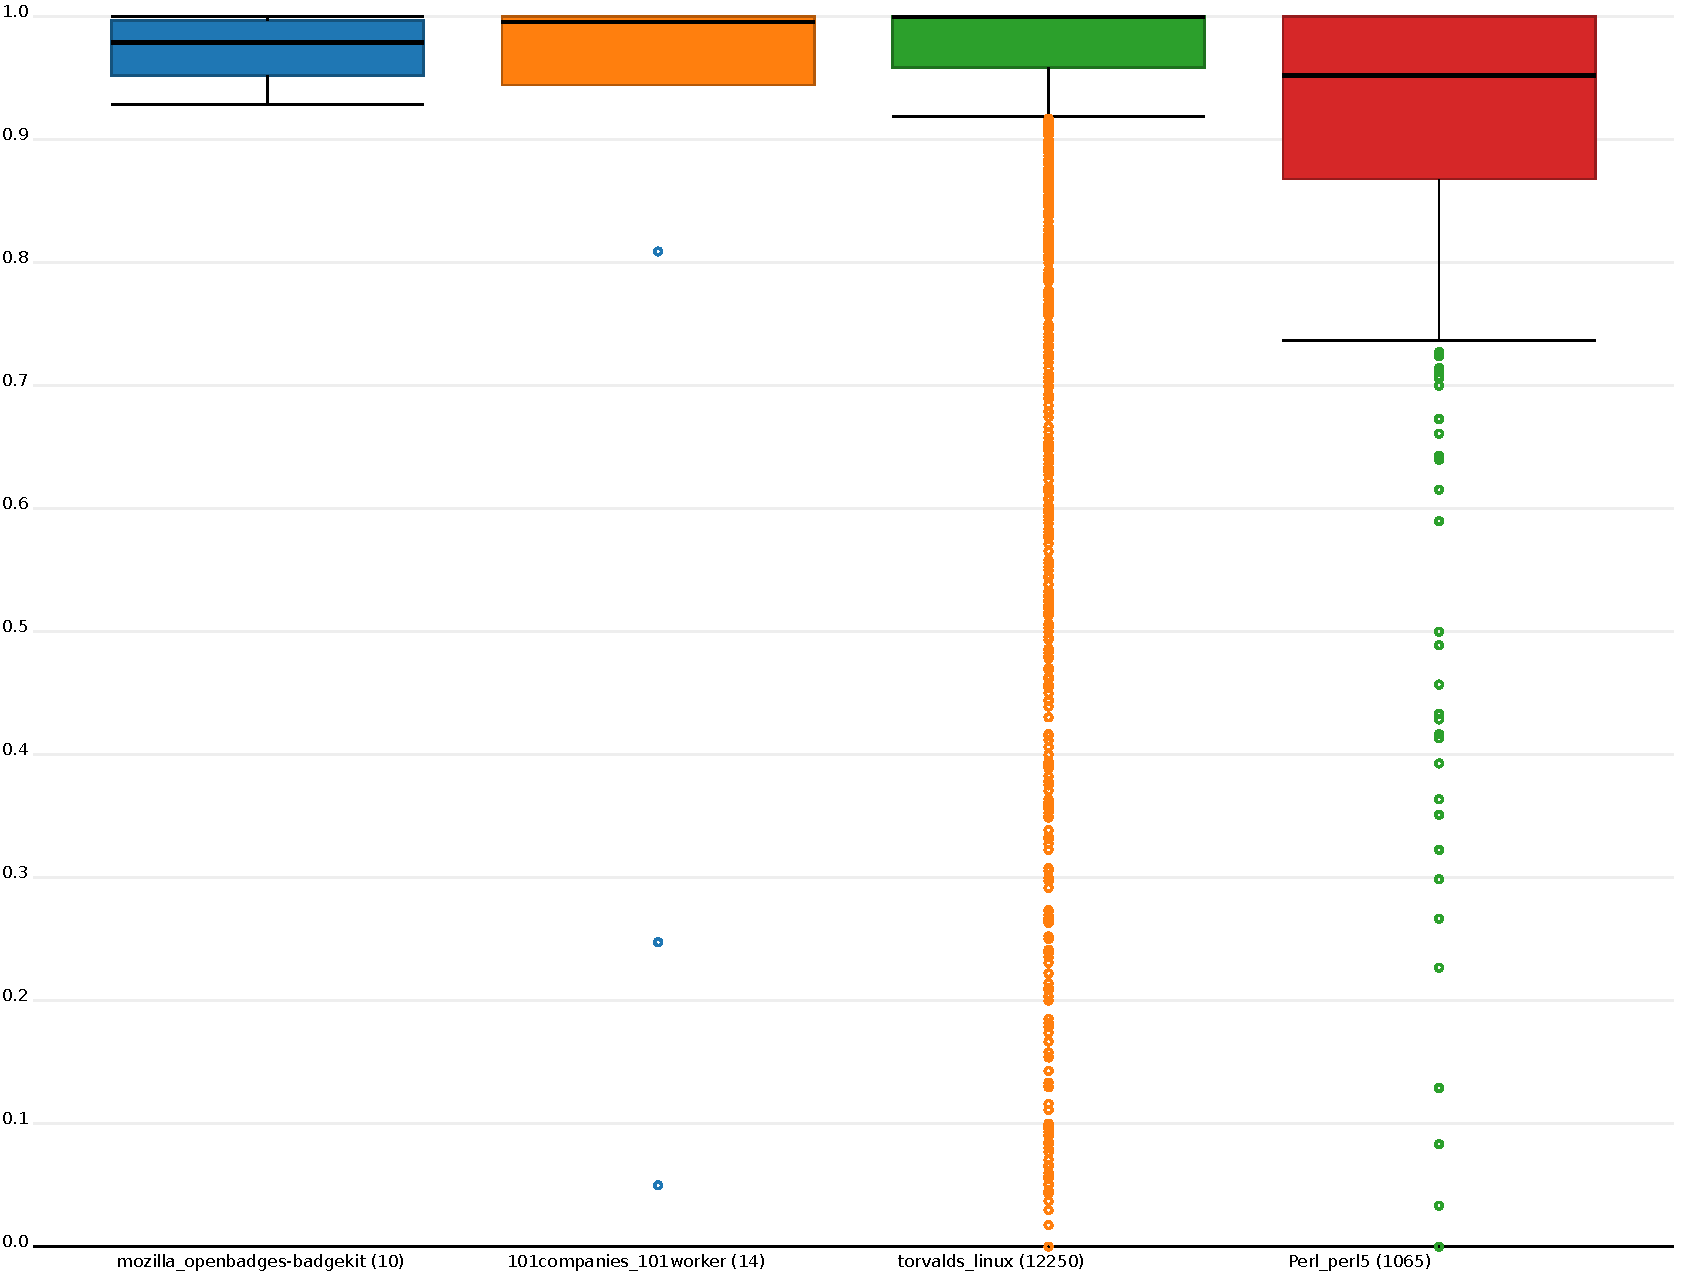
\includegraphics[width=0.8\textwidth]{img/no_period_subject.pdf}
    \caption{No Period Subject Boxplot}
    \label{fig:bp_no_period_subject}
\end{figure}

Finally, figure \ref{fig:bp_no_period_subject} shows that generally none of the repositories put a period at the end of the subject line. This means, that this criterion could be disregarded, if similar behaviour can be observed in other repositories.

The boxplots for the other criteria are available in our Git and were not included here in order to save space.

Based on these results, it is surprisingly hard to draw justified conclusions and answer our first research question positively. While the linux kernel is certainly the most high-profile Git repository in our selection and one might expect a high commit quality from the contributing authors, considering the median it is outperformed in four of thirteen criteria by the other repositories.

Since we lack further objective judgements on the ``goodnes'' of commits or repositories, we can not evaluate if meeting our criteria means having ``good'' commits.

On the other hand, it can be argued that meeting the seven official criteria means having good commits \emph{per definition}, since they have been taken from the official guidelines, and are therefore themselves the missing objective judgement.

In summary, while the analysis results are certainly interesting to look at, they offer no unambiguous answer to our first research question.

\subsection{Machine Learning}
\label{sec:results2}

As an attempt to validate our own criteria, we performed association analysis using the data mining and machine learning software Weka\cite{Weka}. The data set is a commit-level view (see section \ref{subs:Commit-level}) of all rated commits of our sample repositories (see section \ref{sec:data-extraction}). The raw ARFF\footnote{\url{http://www.cs.waikato.ac.nz/ml/weka/arff.html}} data can be found at \url{https://github.com/hartenfels/Commit-Rater/tree/master/samples}.

\begin{table}[t]
    \begin{tabularx}{\textwidth}{|c|X|}\hline
        \textbf{Expected Correlation} & \textbf{Reason} \\\hline
        empty\_second\_line $\Rightarrow$ body\_used & If there is more than one line, the body was used, per our definition. Note that a nonexistent empty line does not count as empty, see section \ref{subs:empty_second_line}.\\\hline
        short\_message $\Leftrightarrow$ $\neg$ long\_message & Obviously, a message cannot have 2 or less and 10 or more words at the same time. \\\hline
        body\_limit $\Rightarrow$ body\_used & Only if the body exists will the body limit criterion be defined. See section \ref{subs:body_limit}. \\\hline
        short\_message $\Rightarrow$ subject\_limit & If two or less words are used in the subject line, it is unlikely that it will be longer than 50 characters. \\\hline
        long\_message $\Rightarrow$ $\neg$ subject\_limit & As the inverse of the above, it is unlikely that 10 or more words can be crammed in a 50 character subject line. \\\hline
    \end{tabularx}
    \caption{Expected correlations, ordered by obviousness}
    \label{tab:expect}
\end{table}

To find an appropriate algorithm, we chose a set of obvious correlations, listed in table \ref{tab:expect}. An algorithm detecting these correctly should also be suitable to detect other non-obvious correlations in our data set.

While almost all attributers built into Weka provided useful output regarding above criteria, we eventuall chose to use the ``Apriori'' attributer\cite{FastWeka,ClassWeka}, as it correctly handled boolean values and did not require the results to be classified. No special parameters are used to call the attributer, only the number of output results has been increased from 10 to 300\footnote{The code to call the attributer can be found at \url{https://github.com/hartenfels/Commit-Rater/blob/master/runweka\#L9}}. The results have been ordered by confidence of their correctness and can be found at \url{https://github.com/hartenfels/Commit-Rater/blob/master/samples/sample\_repos.arff.weka}.

However, only one of our expected criteria can be found in the result set. Two thirds of all results also relate to the no\_misspelling criterion, which, as predicted in section \ref{subs:no_misspelling}, has proven problematic. The same occurs with the no\_vulgarity predictate, which is simply too often true and therefore not a useful criterion. Additionally, some criteria, such as no\_bulk\_changes, cannot be correlated with any other criteria, as they have no connection with any of them.

Due to this sobering result, the research question ``Is Our Personally Chosen Criteria Valid?'' from section \ref{sec:rq2} can clearly be answered by ``no''. The implementation of spell checking does not provide correct results and the vulgarity checking is not actually useful, as there aren't enough commits that fail the check. On the upside, the process of performing this attribution has revealed these issues very clearly, allowing us to correct them and test our corrections by another round of attributions.

Additionally, this machine learning process is not useful for all criteria, as not all of them have a relation to at least one other criterion. Therefore, either more criteria is needed to fill these gaps, or a different way of validiation needs to be used.


%\noindent
%Summarize results in terms of tables, charts, and other kinds of
%figures.
%
%Explain and interpret the results.
%
%Get back to the research question and make sure that it is explicitly answered.
